% Chapter Template

\chapter{Developments} % Main chapter title

\label{Chapter6} % Change X to a consecutive number; for referencing this chapter elsewhere, use \ref{ChapterX}

\lhead{Chapter 6. \emph{Developments}} % Change X to a consecutive number; this is for the header on each page - perhaps a shortened title

%----------------------------------------------------------------------------------------
%	SECTION 1
%----------------------------------------------------------------------------------------

\section{Development Tools}

Development tools used to create an application of counting sheets of cloth are shown in Figure \ref{fig:f601} The tools include MATLAB, Xcode, and OpenCV library. The proposed algorithms are first developed under MATLAB and then implemented in the iPhone using Xcode and OpenCV.
\begin{figure}[t]
	\centering
	\begin{subfigure}[b]{0.2\textwidth}
		
\includegraphics[width=\textwidth]{f601a.png}
		\caption{}\label{fig:f601a}
	\end{subfigure}
	\begin{subfigure}[b]{0.2\textwidth}
		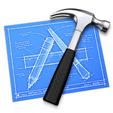
\includegraphics[width=\textwidth]{f601b.png}
		\caption{}\label{fig:f601b}
	\end{subfigure}
	\begin{subfigure}[b]{0.2\textwidth}
		
\includegraphics[width=\textwidth]{f601c.png}
		\caption{}\label{fig:f601c}
	\end{subfigure}
	\caption{(a) MATLAB (b) Xcode (c) OpenCV}
	\label{fig:f601}
	
\end{figure}
%-----------------------------------
%	SUBSECTION 1
%-----------------------------------
\subsection{MATLAB}
MATLAB is a tool used to develop and test algorithms. There is an image processing toolbox provided in MATLAB which can be used to achieve the tasks.

%-----------------------------------
%	SUBSECTION 2
%-----------------------------------

\subsection{Xcode}
Xcode is a tool used for developing application for OS X and iOS platform. This project uses Xcode to implement the algorithms developed by using MATLAB together with OpenCV library. The tool can then be used to create an application on iPhone.

%-----------------------------------
%	SUBSECTION 3
%-----------------------------------
\subsection{OpenCV}
OpenCV library is image processing in C++ language library. It is function that similar image processing in MATLAB program. In this project use OpenCV library to apply the algorithm that provide by MATLAB program. 

%----------------------------------------------------------------------------------------
%	SECTION 2
%----------------------------------------------------------------------------------------

\section{Project Implementation}
The implementation of this project is separated into two major parts, i.e. application part and algorithm part. Application part is implemented using Objective-C language on Xcode. The aim of this part is to develop a friendly user interface and image preprocessing. The application development part is defined to be the part concerning user interface development and iOS based device implementation. This part uses Xcode to create an application based on iOS platform with OpenCV library. The algorithms development part develops and test the algorithm using MATLAB as a tool. The developed algorithm is then transferred to be used in the application development part.
%----------------------------------------------------------------------------------------
%	SECTION 3
%----------------------------------------------------------------------------------------
\section{Application Development Part}
Application development part develops user interface of the application for counting sheets of cloth. The user interface is developed by using Objective-C in Xcode. The user interface is designed as follows Figure \ref{fig:f603}. Consider Figure \ref{fig:f603} at the left, the application name is displayed on top of frame. At center, it is an input image area which displays the input image from gallery or camera. There are two lower left buttons, i.e. gallery button and camera button. Both buttons refer to an input image buttons.
\begin{itemize}
	\item{\textbf{Gallery Button:} this button specifies the device’s photo library.}
	\item{\textbf{Camera Button:} this button specifies the device’s built-in camera.}
\end{itemize}
\begin{figure}[t]
	\centering
	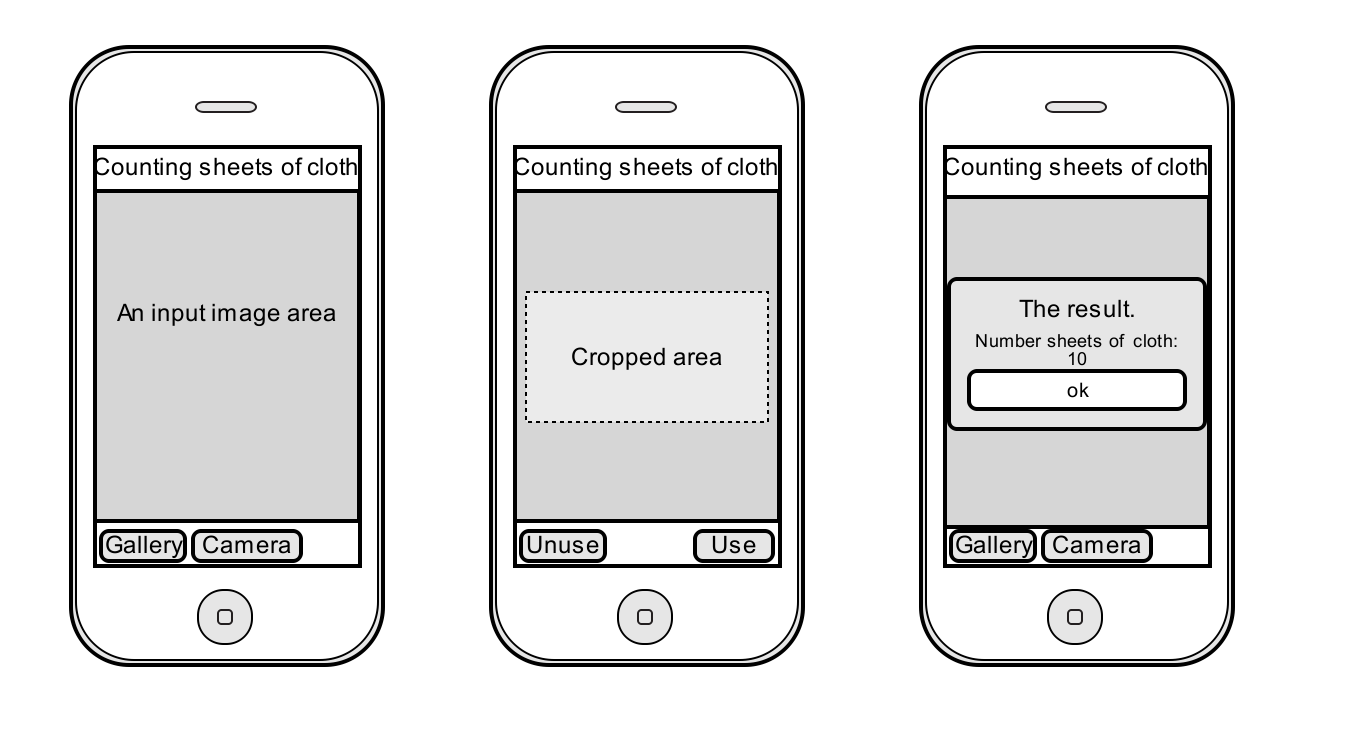
\includegraphics[scale=0.3]{f603.png}
	\caption{Designed Moqup}
	\label{fig:f603}
\end{figure}
After obtained an input image, user crops an input image in cropped area which is area fixed. But the input image can be resized as shown in Figure \ref{fig:f603} at the middle. There are two lower left and right buttons, i.e. unused button and use button.
\begin{itemize}
	\item{\textbf{Unuse Button:} the input image will be retaken.}
	\item{\textbf{Use Button:} the input image will be cropped in cropped area.}
\end{itemize}
After the input image is cropped, a system will alert a result message as shown in Figure \ref{fig:f603} at the right.

In order to apply the application algorithm from MATLAB, Objective-C will be used OpenCV library to creates algorithm with image processing technique.

%----------------------------------------------------------------------------------------
%	SECTION 4
%----------------------------------------------------------------------------------------
\section{Algorithm Development Part}
The algorithm development aims to develop algorithm that can count the sheets of cloth from an input image. The overview algorithms developed in this project is shown in Figure \ref{fig:f602}.
\begin{figure}[t]
	\centering
	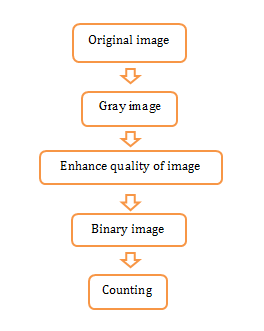
\includegraphics[scale=1]{f602.png}
	\caption{Flow of algorithm}
	\label{fig:f602}
\end{figure}

There are five steps to achieve the counting result: receive an input image (Original image box), preprocessing the image (Gray image box, Enhance quality of image box, Binary image box) and display the number of sheets of cloth (Counting box).

%-----------------------------------
%	SUBSECTION 4-1
%-----------------------------------
\subsection{RGB to Gray-scale Image Conversion}
This part of the algorithm converts a RGB image into a gray-scale image. The process starts by selecting an original input image from the image gallery or the one taken by camera. An example of the input image is shown in Figure \ref{fig:f604a}. The original input image is then converted into the gray-scale image as shown in Figure \ref{fig:f604b}. 
\begin{figure}[t]
	\centering
	\begin{subfigure}[b]{0.3\textwidth}
		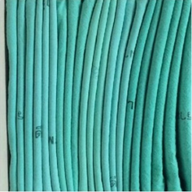
\includegraphics[width=\textwidth]{f604a.png}
		\caption{}\label{fig:f604a}
	\end{subfigure}
	\begin{subfigure}[b]{0.3\textwidth}
		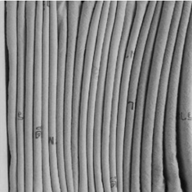
\includegraphics[width=\textwidth]{f604b.png}
		\caption{}\label{fig:f604b}
	\end{subfigure}
	\caption{(a) An original image (b) Gray-scale image}
\end{figure}
%-----------------------------------
%	SUBSECTION 4-2
%-----------------------------------
\subsection{Image Quality Enhancement}
This step is used to improve contrast of an image Figure \ref{fig:f606} illustrates the result after applying the enhancement algorithm. In MATLAB, the function used for contrast adjustment is called adpthisteg. The detail of this method is discussed previously in section \ref{sec:3.4}. In application part, the contrast of the gray-scale image is improved by using the function from OpenCV library, i.e. histogram equalization (discuss in section \ref{sec:3.1}).
\begin{figure}[t]
	\centering
	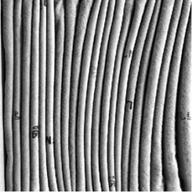
\includegraphics[scale=1]{f605.png}
	\caption{Result of image enhancement}
	\label{fig:f605}
\end{figure}

%-----------------------------------
%	SUBSECTION 4-3
%-----------------------------------

\subsection{Binary Image Conversion}
The gray-scales image that already enhanced the contrast in image is converted into binary image as shown in Figure \ref{fig:f606}. After conversion, the result binary image possesses two intensity values 1 or 0. In MATLAB, the conversion of gray-scales image to binary image used im2bw function. The im2bw function converts an RGB image to binary image (discus in section \ref{sec:3.5}). In Objective-C, gray-scales image is converted to binary image using Otsu thresholding with functionally \textit{cv::threshold()}  (discus in section \ref{sec:3.2}).
\begin{figure}[t]
	\centering
	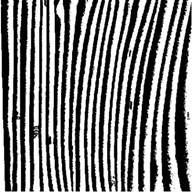
\includegraphics[scale=1]{f606.png}
	\caption{Binary image}
	\label{fig:f606}
\end{figure}

%-----------------------------------
%	SUBSECTION 4-4
%-----------------------------------
\subsection{Counting}
This section discusses about counting algorithm that counts the sheets of cloth from binary image. The algorithm divides the binary image into ten parts using ten horizontal straight lines Figure \ref{fig:f609a}. Each black straight line contains intensity values which are stored in an array. An example of intensity values contained in the array corresponding to each straight line is shown in Figure \ref{fig:f607}.
\begin{figure}[t]
	\centering
	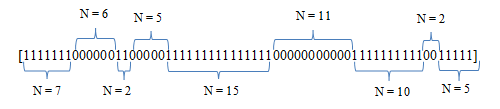
\includegraphics[scale=1]{f607.png}
	\caption{Intensity value in array}
	\label{fig:f607}
\end{figure}

Elements in array flip from one to zero and zero to one where the number of N less than five where N refers to the length of the series of 0 or 1. The intensity values are altered in two locations marked as underline in Figure \ref{fig:f608}.
\begin{figure}[t]
	\centering
	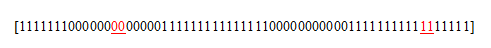
\includegraphics[scale=1]{f608.png}
	\caption{Improved intensity value in array}
	\label{fig:f608}
\end{figure}
From the array of 0 and 1 shown in Figure \ref{fig:f608}, the result of counting sheets of cloth is three sheets. This counting result will be kept and used in the later processing.

By using this method each horizontal straight line produces series of black and white strips. Figure \ref{fig:f609a} illustrates the binary image with ten horizontal straight lines superimpose on it while Figure \ref{fig:f609b} shows the result after applying the algorithm to the first line.
\begin{figure}[t]
	\centering
	\begin{subfigure}[b]{0.3\textwidth}
		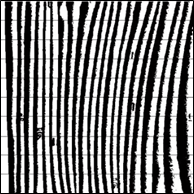
\includegraphics[width=\textwidth]{f609a.png}
		\caption{}\label{fig:f609a}
	\end{subfigure}
	\begin{subfigure}[b]{0.3\textwidth}
		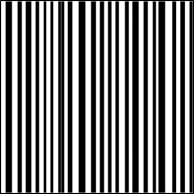
\includegraphics[width=\textwidth]{f609b.png}
		\caption{}\label{fig:f609b}
	\end{subfigure}
	\caption{(a) Binary image with ten (b) New binary image resulted from the first horizontal straight line}
\end{figure}

This chapter presents all development tools and implementation application. After that an evaluation will be explained in next chapter.